\documentclass[journal]{IEEEtran}

% ---------- Engine & fonts ----------
\usepackage{iftex}
\ifXeTeX
  \usepackage{fontspec}
  \usepackage{xeCJK}
  % English fonts (TeX Gyre family)
  \setmainfont{TeX Gyre Termes}
  \setsansfont{TeX Gyre Heros}
  \setmonofont{TeX Gyre Cursor}
  % Japanese fonts (Noto CJK)
  \setCJKmainfont{Noto Serif CJK JP}
  \setCJKsansfont{Noto Sans CJK JP}
\fi

% ---------- Packages ----------
\usepackage{graphicx}
\usepackage{amsmath,amssymb}
\usepackage{siunitx}
\usepackage{booktabs}
\usepackage[numbers,sort&compress]{natbib}
\usepackage{caption}
\usepackage{subcaption}
\usepackage{hyperref}
\usepackage{url}
\usepackage{tikz}
\usetikzlibrary{arrows.meta,positioning,fit,calc}
\usepackage{pgfplots}
\pgfplotsset{compat=1.18}

% ---------- Helper: safe \input ----------
\makeatletter
\newcommand{\maybeinput}[1]{%
  \IfFileExists{#1}{\input{#1}}{\textit{[missing: #1]}}%
}
\makeatother

% ---------- Begin Document ----------
\begin{document}

\title{FeFET CMOS 0.18\,$\mu$m Integration Study}
\author{Samizo-AITL}
\maketitle

% ================= Abstracts =================
\begin{abstract}
\maybeinput{build/abstract_en.tex}
\end{abstract}

\begin{IEEEkeywords}
FeFET, HfZrO$_x$, 0.18\,$\mu$m CMOS, reliability, process integration
\end{IEEEkeywords}

\section*{要旨}
\maybeinput{build/abstract_ja.tex}

\section*{索引用語}
FeFET,強誘電 HfZrO$_x$,0.18\,$\mu$m CMOS,信頼性,プロセス統合

% ================= Body =================
\section{Introduction}
\maybeinput{build/intro_en.tex}

\section*{序論}
\maybeinput{build/intro_ja.tex}

% =========================================================
% Process Integration
% =========================================================
\section{Process Integration}

% ---- TikZ Flow ----
\begin{figure}[t]
\centering
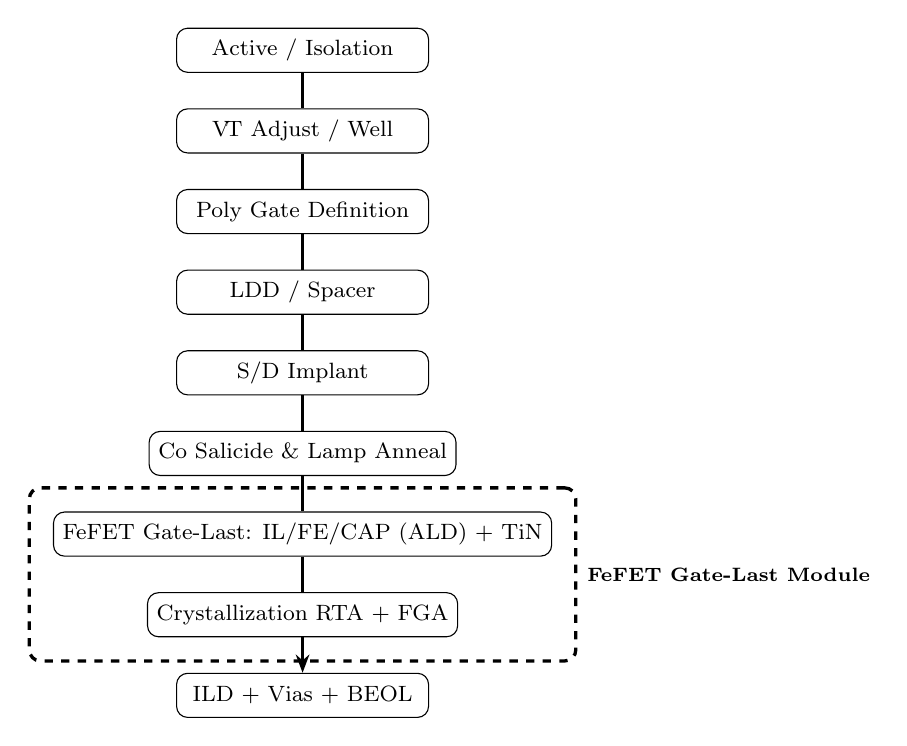
\begin{tikzpicture}[
  node distance=4.5mm,
  stage/.style={draw,rounded corners,minimum width=32mm,minimum height=5.6mm,align=center,font=\footnotesize},
  arr/.style={-{Stealth},thick},
  ann/.style={font=\scriptsize}
]
\node[stage] (act)  {Active / Isolation};
\node[stage,below=of act] (vt)  {V\!T Adjust / Well};
\node[stage,below=of vt]  (poly) {Poly Gate Definition};
\node[stage,below=of poly] (ldd)  {LDD / Spacer};
\node[stage,below=of ldd]  (imp)  {S/D Implant};
\node[stage,below=of imp]  (sal)  {Co Salicide \& Lamp Anneal};
\node[stage,below=of sal]  (fegate)  {FeFET Gate-Last: IL/FE/CAP (ALD) + TiN};
\node[stage,below=of fegate]  (rta)  {Crystallization RTA + FGA};
\node[stage,below=of rta]  (ild)  {ILD + Vias + BEOL};

\draw[arr] (act) -- (vt) -- (poly) -- (ldd) -- (imp) -- (sal) -- (fegate) -- (rta) -- (ild);

\node[draw,dashed,very thick,rounded corners,fit=(fegate) (rta),inner sep=3mm,
      label={[ann]right:\textbf{FeFET Gate-Last Module}}] {};
\end{tikzpicture}
\caption{Placement of FeFET module within the 0.18\,$\mu$m CMOS baseline.}
\label{fig:flow}
\end{figure}

% ---- Mask/step table ----
\begin{table}[t]
  \centering
  \caption{Added masks / process steps relative to baseline logic.}
  \label{tab:masks}
  \begin{tabular}{@{}lcc@{}}
    \toprule
    \textbf{Step} & \textbf{Mask} & \textbf{Comment}\\
    \midrule
    FE metal gate & +1 & Shared / reuse analog option route\\
    FE anneal     &  0 & Done in BEOL furnace (no extra mask)\\
    \bottomrule
  \end{tabular}
\end{table}

\maybeinput{build/process_integration_en.tex}
\section*{プロセス統合}
\maybeinput{build/process_integration_ja.tex}

% =========================================================
% Reliability
% =========================================================
\section{Reliability}

% ---- Endurance ----
\begin{figure}[t]
\centering
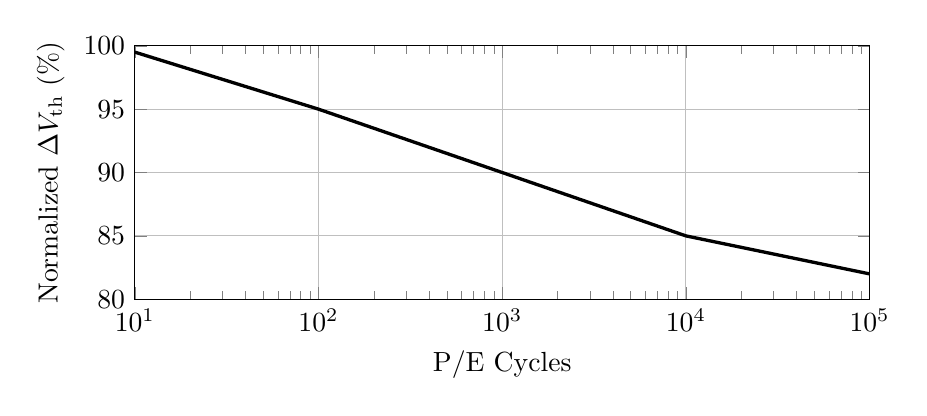
\begin{tikzpicture}
\begin{semilogxaxis}[
  width=0.9\linewidth, height=48mm,
  xlabel={P/E Cycles}, ylabel={Normalized $\Delta V_{\mathrm{th}}$ (\%)},
  ymin=80, ymax=100, xmin=10, xmax=1e5,
  ymajorgrids, xmajorgrids
]
\addplot[very thick] coordinates {(10,99.5) (100,95.0) (1e3,90.0) (1e4,85.0) (1e5,82.0)};
\addplot[densely dashed] coordinates {(10,80) (1e5,80)};
\end{semilogxaxis}
\end{tikzpicture}
\caption{Endurance under ±2.5\,V, 10\,$\mu$s program/erase pulses.}
\label{fig:endurance}
\end{figure}

% ---- Wake-up & Retention ----
\begin{figure}[t]
\centering
\begin{subfigure}{0.45\linewidth}
\centering
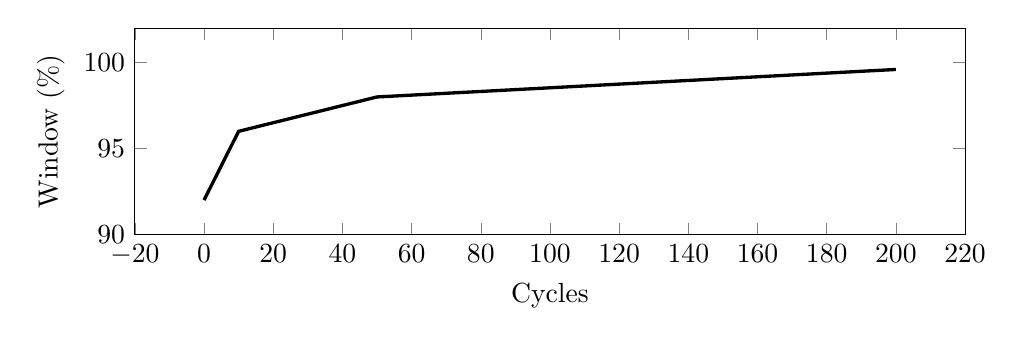
\begin{tikzpicture}
\begin{axis}[width=\linewidth, height=42mm, xlabel={Cycles}, ylabel={Window (\%)}, ymin=90, ymax=102]
\addplot[very thick] coordinates {(0,92) (10,96) (50,98) (200,99.6)};
\end{axis}
\end{tikzpicture}
\caption{Wake-up}
\end{subfigure}\hfill
\begin{subfigure}{0.45\linewidth}
\centering
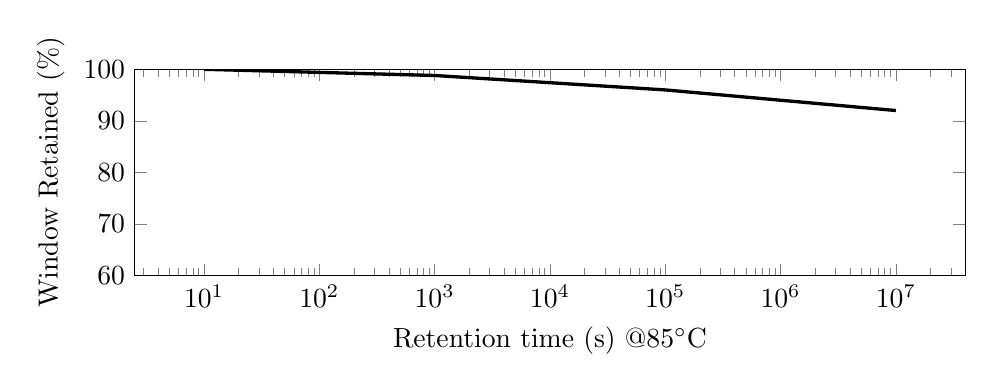
\begin{tikzpicture}
\begin{semilogxaxis}[width=\linewidth, height=42mm, xlabel={Retention time (s) @85$^\circ$C}, ylabel={Window Retained (\%)}, ymin=60, ymax=100]
\addplot[very thick] coordinates {(1e1,100) (1e3,98.8) (1e5,96) (1e7,92)};
\end{semilogxaxis}
\end{tikzpicture}
\caption{Retention}
\end{subfigure}
\caption{Wake-up and retention characteristics.}
\end{figure}

% ---- TDDB ----
\begin{figure}[t]
\centering
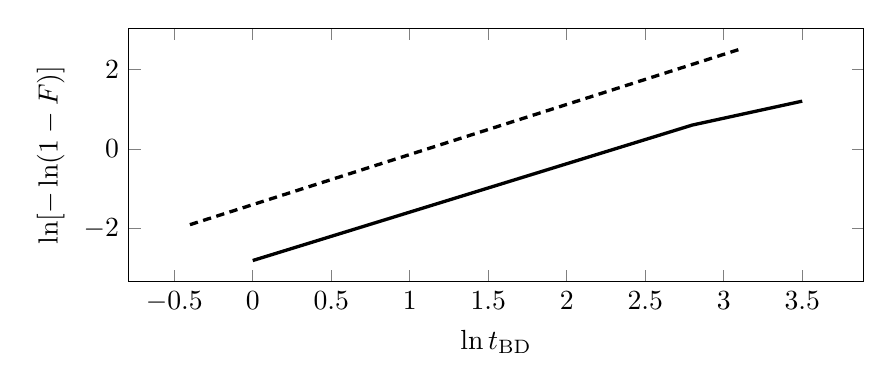
\begin{tikzpicture}
\begin{axis}[width=0.9\linewidth, height=48mm, xlabel={$\ln t_{\mathrm{BD}}$}, ylabel={$\ln[-\ln(1-F)]$}]
\addplot[very thick] coordinates {(0,-2.8) (2.8,0.6) (3.5,1.2)};
\addplot[densely dashed, very thick] coordinates {(-0.4,-1.9) (3.1,2.5)};
\end{axis}
\end{tikzpicture}
\caption{TDDB Weibull representation at two stress fields.}
\label{fig:tddb}
\end{figure}

\maybeinput{build/reliability_en.tex}
\section*{信頼性}
\maybeinput{build/reliability_ja.tex}

% =========================================================
% Conclusion
% =========================================================
\section{Conclusion}
\maybeinput{build/conclusion_en.tex}
\section*{結論}
\maybeinput{build/conclusion_ja.tex}

% ================= References =================
\bibliographystyle{IEEEtran}
\bibliography{refs}

% ================= Biography =================
\section*{Author Biography}
Shinichi Samizo received the M.S. degree in Electrical and Electronic Engineering from Shinshu University, Japan.  
He joined Seiko Epson Corporation in 1997, where he engaged in semiconductor device process development including 0.25--0.18\,$\mu$m CMOS, HV-CMOS, DRAM, FeRAM, and FinFET/GAA.  
He also contributed to inkjet MEMS process and thin-film piezo actuator design, leading to the productization of PrecisionCore printheads.

\section*{著者略歴}
三溝真一(Shinichi Samizo) 信州大学大学院 電気電子工学専攻 修了。  
1997年よりセイコーエプソン株式会社にて、0.25~0.18\,$\mu$m CMOS、HV-CMOS、DRAM、FeRAM、FinFET/GAAの開発に従事。  
また、インクジェットMEMSプロセス開発、薄膜ピエゾアクチュエータ設計、PrecisionCoreプリントヘッドの量産化に携わった。

\end{document}
